\documentclass[ba]{imsart}

% \documentclass[ba,preprint]{imsart}% use this for supplement article
\usepackage{amsmath}
\usepackage{amssymb}
\usepackage{amsfonts}
\usepackage{amsthm}
%% \usepackage{amsaddr}


\usepackage{thm-restate}
\usepackage{tikz,pgfplotstable}
\usetikzlibrary{patterns}
\pgfplotsset{compat=1.9} % set to 1.8 to get old behaviour
%\usepackage{hyperref}

\newcommand{\R}{\ensuremath{\mathbb{R}}}
\newcommand{\eps}{\varepsilon}
\newcommand{\M}{\mathcal{M}}

\newcommand{\der}{\text{\textup{d}}}
\newcommand{\diag}{\textup{diag}}

\providecommand{\x}{}
\renewcommand{\x}{\mathbf{x}}
\newcommand{\y}{\mathbf{y}}

\newcommand{\hil}{\mathcal{H}}
\newcommand{\hilp}{\mathcal{H}_p}
\newcommand{\hilo}{\mathcal{H}_o}
\newcommand{\obs}{\mathcal{O}}
\newcommand{\pobs}{\mathcal{P}}
\newcommand{\fwd}{\mathcal{F}}

\newcommand{\obsm}{\widehat{\obs}}
\newcommand{\Sigmam}{\widehat{\Sigma}}
\newcommand{\postcovm}{\widehat{\Gamma_{\textup{post}}}}
\newcommand{\uu}{\mathbf{u}}
\newcommand{\tar}{\Psi}
\DeclareMathOperator*{\argmin}{arg\,min}
\DeclareMathOperator*{\argmax}{arg\,max}

% Definitions for second chapter
\newcommand{\data}{\mathbf{d}}
\newcommand{\param}{\mathbf{m}}
\newcommand{\normal}{\mathcal{N}}
\newcommand{\pr}{\mu_{\textup{pr}}} %Prior measure
%\newcommand{\post}{\mu_{\textup{post}}^{\data, \obs}} % Posterior measure
\newcommand{\post}{\mu_{\textup{post}}} % Posterior measure for slides
\newcommand{\prmean}{\param_{\textup{pr}}} % Prior mean
\newcommand{\postmean}{\param_{\textup{post}}} % Posterior mean
\newcommand{\postcov}{\Gamma_{\textup{post}}} % Posterior covariance
\newcommand{\prcov}{\Gamma_{\textup{pr}}} % Prior covariance
\newcommand{\modcov}{\Gamma_{\textup{model}}} % Model covariance
\newcommand{\tmp}{\mathcal{G}}
\newcommand{\meas}{\mathbf{o}}
\newcommand{\ev}{\mathbf{e}} % eigenvector 
\newcommand{\func}{\mathbf{a}}
\newcommand{\tr}[1]{\textup{tr}\left \{#1 \right \} }
\newcommand{\ttr}[1]{\textup{tr}\ #1}
\newcommand{\rank}{\textup{rank}\ }
\newcommand{\des}{\eta} % vector of design parameters
\newcommand{\sigsqr}{\sigma^2}

%% \newcommand{\opt}{\mathfrak{D}}
\newcommand{\opt}{\mathcal{D}}
\newcommand{\postopt}{\mu_{\textup{post}}^{\data, \opt}} % Posterior measure

%% %\usepackage{comment}% http://ctan.org/pkg/comment
%% %% %% %\excludecomment{proof}
%% %% \excludecomment{figure}
%% %% \let\endfigure\relax


%% %\overfullrule=0pt

\theoremstyle{plain}
\newtheorem{theorem}{Theorem}
\newtheorem{corollary}[theorem]{Corollary}
\newtheorem{lemma}[theorem]{Lemma}
\newtheorem{proposition}[theorem]{Proposition}
\theoremstyle{definition}
\newtheorem{definition}[theorem]{Definition}
\newtheorem{example}[theorem]{Example}
\newtheorem{conjecture}[theorem]{Conjecture}
\theoremstyle{remark}
\newtheorem{remark}[theorem]{Remark}
%
\pubyear{2021}
\volume{TBA}
\issue{TBA}
% \doi{0000}
%\arxiv{}
\firstpage{1}
\lastpage{1}

\usepackage{amsthm}
\usepackage{amsmath}
\usepackage{natbib}
\usepackage[colorlinks,citecolor=blue,urlcolor=blue,filecolor=blue,backref=page]{hyperref}
\usepackage{graphicx}

\startlocaldefs
% ** Local definitions **
\endlocaldefs

\begin{document}

%% *** Frontmatter *** 

\begin{frontmatter}
\title{Measurement Clusterization in Bayesian D-optimal Designs in Infinite Dimensions}

%\title{\support{}}
\runtitle{Measurement Clusterization in D-optimal Designs}
%\author{Yair Daon}
%\numberwithin{equation}{section}

\begin{aug}
\author{\fnms{Yair} \snm{Daon}\thanksref{addr1}\ead[label=e1]{yair.daon@gmail.com}}
\runauthor{Yair Daon}

\address[addr1]{Azrieli Faculty of Medicine, Bar-Ilan University, Safed, Israel
    \printead{e1} % print email address of "e1"
}

\end{aug}

\begin{abstract}
Estimation of parameters in physical processes often demands costly measurements, prompting the pursuit of an optimal measurement strategy. Finding such strategy is termed the problem of \emph{optimal experimental design}, abbreviated as optimal design. Remarkably, optimal designs can yield tightly clustered measurement locations, leading researchers to fundamentally revise the design problem just to circumvent this issue. Some authors introduce error correlation among error terms that are initially independent, while others restrict measurement locations to a finite set of locations. While both approaches may prevent clusterization, they also fundamentally alter the optimal design problem.

In this study, we consider Bayesian D-optimal designs, i.e.~designs that maximize the expected Kullback-Leibler divergence between posterior and prior. We propose an analytically tractable model for D-optimal designs over Hilbert spaces. In this framework, we make several key contributions: \textbf{(a)} We establish that measurement clusterization is a generic trait of D-optimal designs with independent Gaussian measurement errors, and prove that introducing correlations among measurement error terms mitigates clusterization. \textbf{(b)} We characterize D-optimal designs as reducing uncertainty across a subset of prior covariance eigenvectors. Finally, \textbf{(c)} We leverage this characterization to argue that measurement clusterization arises as a consequence of the pigeonhole principle: when more measurements are taken than there are locations where the select eigenvectors are large and others are small --- clusterization occurs. 
%
%% In summary, in this study we shed light on an often ignored issue with
%% Bayesian D-optimal designs. We characterize such designs and show why
%% clusterization arisesit arisestheir inherent properties, propose
%% strategies to address clusterization, and provide insights into the
%% fundamental attributes underlying measurement design optimization.
\end{abstract}

%% ** Keywords **
\begin{keyword}[class=MSC]
\kwd[Primary ]{62F15}
\kwd{35R30}
\kwd[; secondary ]{28C20}
\end{keyword}

\end{frontmatter}

\section{Introduction}\label{section:intro}
The practice of experimental design entails specifying every detail of
running an experiment \cite{chaloner1995} and at its simplest form,
experimental design involves choosing a set of measurements to be
taken. For example, consider the process of searching for oil:
measuremnts require digging holes in the ground and a \emph{design}
simply indicates which holes should be dug
\cite{horesh2008borehole}. Since measurements are expensive, only a
limited number of measuremnts can be taken, and thus carefully
choosing measuremt locations is crucial.

Specifiyng the right set of measurements holds particular significance
when solving an \emph{inverse problem} --- i.e.~making inference of
the physical world utilizing a physical model of a phenomenon of
interest \cite{tarantola2005,kaipio2005}. In an inverse problem, we
seek to infer physical quantities, based on observations and a model
of the physical world. Models are typically phrased in the language of
ordinary or partial differential equations.

Inverse problems are ubiquitous in science and engineering. For
example, in electrical impedance tomography (EIT) we seek to infer the
structure of the inside of a human body. Inference is conducted based
on observations of electrical current impedance measured at specific
electrode locations on the skin, leveraging known equations of
electric current flow \cite{horesh2010impedance}. Magnetic Resonance
Imaging (MRI) also entails solving an inverse problem. There,
radio-frequency pulses are sent through the human body in the presence
of a strong magnetic field. The response of one's body contents to
these radio-frequency pulses is measured, allowing a radiologist to
view the internals of a body in a noninvasive manner
\cite{horesh2008mri}. An inverse problem also arises in oil and gas
exploration, where acoustic waves are sent through "boreholes" ---
deep cylindrical wells drilled into the ground. Data of travel and
return times of the acoustic waves are recorded. Wave travel and
return time is influenced by the properties of the subsurface
materials, such as density, elasticity, and the presence of fluids or
voids. Combining travel time data with a geophisical models of
contents of the earth's crust facilitates reconstructing the structure
of the subsurface in a process called \emph{borehole tomography}
\cite{horesh2008borehole}. Inverse problems also arise in many other
areas of seismology and geology \cite{rabinowitz1990, steinberg1995}
and medical imaging \cite{tarantola2005}. In many inverse problems the
goal is to infer some numerical parameter. However, in the formulation
we consider in this study, as well as in the examples above, the goal
is to conduct inference over some \emph{function} over $\Omega$, where
\(\Omega \subseteq \mathbb{R}^d, d=1,2,3\) is a spatial domain of
interest.

\subsection{D-optimal Designs}\label{subsec:D}
In all of the examples of inverse problems we have seen, as well as in
many other applications, only a limited number of measurements are
allowed. For example, in borehole tomography, a measurement involves
drilling a deep well in the ground --- a very costly endeavor. Even in
a seemingly simpler application such as MRI, a patient cannot occupy
the MRI machine for too long, hence only a limited number of
measurements can be taken. Therefore, measurements should be chosen to
most benefit the user. Typically, a user will consider some utility,
called a \emph{design criterion} and take measurements that maximize
this utility. Two of the most widely recognized and extensively
studied design criteria are A- and D-optimality.

In this study, we focus on the Bayesian D-optimality
criterion. Bayesian D-optimality carries a simple and intuitive
meaning: measurements chosen according to the D-optimality criterion
maximize the expected Kullback-Liebler (KL) divergence from posterior
to prior \cite{chaloner1995, AlexanderianGloorGhattas14,
  CoverThomas91}. Utilizing KL divergence for quantifying differences
between distributions is standard practice and we will not motivate it
further here. For a discrete parameter $\param$ and data $\data$, the
KL divergence is defined as
\begin{equation}\label{eq:basic KL}
  D_{KL}\left (\Pr(\param|\data)||\Pr(\param)\right ) =  \sum_{\param} \log
  \frac{\Pr(\param|\data)}{\Pr(\param)} \Pr(\param|\data). 
\end{equation}
Of course, data $\data$ is not known before the experiment is
conducted, so we average over it to define the D-optimality criterion
as:
\begin{equation*}
  \mathbb{E}_{\data}\left [ D_{KL}\left (\Pr(\param|\data)||\Pr(\param)\right ) \right ]
\end{equation*}
We refer to a set of measuremnts that maximizes the D-optimality
criterion as a \emph{D-optimal design}.

For a linear model with Gaussian prior in finite dimensions, a
D-optimal design minimizes the determinant of the posterior covariance
\cite{chaloner1995}. In Section \ref{subsec:D optimal design} we give
a more general definition of the D-optimality criterion that applies
to arbitrary measures. We also show how the D-optimality criterion
generalizes to linear models over infinite-dimensional Hilbert spaces
(i.e.~function spaces).

\subsection{A toy model: the 1D heat equation}\label{subsec:toy}
For concreteness, let us now consider a toy model of a physical
process for which we wish to solve an inverse problem: a partial
differential equation known as the \emph{heat equation} in one
dimension (1D heat equation henceforth). Readers less familiar with
partial differential equations can think of the following setup:
before us there is a perfectly insulated metal rod. At each point on
the rod the temperature is different and unknown, and we call this
temperature distribution the \emph{initial condition}. We wait for a
short time $T$ and let the heat dissipate a bit inside the rod. The
heat equation determines the heat distribution inside the rod at time
$t=T$.

The full time evolution of heat in the rod $\Omega=[0,1]$ is formally
described by the following three equations:
\begin{subequations}%\label{eq:heat equation}
  \begin{alignat}{2}
    u_t &= \Delta u &&\qquad \text{in } [0,1] \times [0,\infty), \label{eq:heat1}\\
    u &= 0 &&\qquad \text{on } \{0, 1\} \times [0,\infty), \label{eq:heat2}\\
    u &= u_0 &&\qquad \text{on }[0,1] \times \{0\}. \label{eq:heat3}
  \end{alignat}
\end{subequations}
As time passes, heat disspates across the rod as hotter regions,
e.g.~local maximas of the heat distribution, become cooler. This
behavior is captured by eq.~\eqref{eq:heat1}: the Laplacian at local
maxima is negative, so $u_t = \Delta u$ implies $u$ decreases at its
maximas, and the reverse happens at local minima. Eq.~\eqref{eq:heat2}
describes the \emph{boundary condition}, which dictates how heat
interacts with the outside world at the two edges of the rod
$\{0,1\}$. Specifically, eq.~\eqref{eq:heat2} implements an absorbing
boundary, i.e.~heat that interacts with the boundary immediately
disappears. This type of boundary condition is known as a
\emph{homogeneous Dirichlet boundary condition}. Eq.~\eqref{eq:heat3}
describes the \emph{initial condition}, i.e.~the heat distribution
inside the rod at time $t=0$.

Solving the 1D heat equation is straightforward. Any initial heat
distribution $u_0\in L^2([0,1])$ that satisfies the homogeneous
Dirichlet boundary condition is a linear combination of sines
$\ev_n(x) = \sin(2\pi n x)$. Now, note that $\ev_n$ are in fact
eigenvectors of the Laplacian: $\Delta \ev_n = -(2\pi n)^2\ev_n$. The
linearity of the Laplacian implies the linearity of the heat equation
and we can solve in Fourier / frequency space. It is important to note
that when solving the heat equation we \emph{invert} the
Laplacian. I.e.~eigenvalues of the linear operator that describes the
time evolution of heat are $(2\pi n)^{-2}$.

In the \emph{inverse problem of the 1D heat equation}, our goal is to
infer the initial condition $u_0 = u(\cdot, 0)$ from observations of
the final condition $u(\cdot, T)$. However, we are not able to measure
$u(\cdot, T)$ at every point in the domain $\Omega$. Rather, we take
some number of temperature measurements on the rod once our waiting
time $T$ has passed and try to infer $u(\cdot, 0)$ from these
measurements.

The inverse problem of the 1D heat equation is difficult ("ill-posed")
since heat spreads in a diffusive manner and any roughness in the
initial condition is quickly smoothed, see Supplementary movies S1 and
S2 (code generating these movies is located in module
\texttt{movies.py} in the accompanying
\href{https://github.com/yairdaon/OED}{repository}). For ill-posed
problems regularization is required, and we implement such
regularization via a fully Bayesian formulation of the inverse
problem.

Specifically, we set a prior on the initial condition $u_0 \sim
\mathcal{N}(0, (-\Delta)^{-1})$, where we impose the homogeneous
Dirichlet boundary condition on the Laplacian. We choose
$(-\Delta)^{-1}$ as our covariance operator following \cite{Stuart10}:
our choice ensures the power of the negative Laplacian inside the
parentheses is larger than $d/2$, where $d=1$ is the dimension of our
computational domain $\Omega$. One can intuitively understand this
choice from Weyl's asymptotics, that states that the eigenvalues of
Laplacian increase as $n^{d/2}$. Thus, our choice of covariance
$(-\Delta)^{-1}$ ensures higher modes decay sufficiently quickly, so
prior samples have sufficient regularity. Our choice of prior
covariance ensures the posterior is well-defined and well-behaved
\cite[Theorem 3.1 and Lemma 6.25]{Stuart10}.

\subsection{Measurement Clusterization}
Surprisingly, A- and D-optimal designs for inverse problems have been
observed to yield remarkably similar measurements in certain cases
\cite{fedorovDesignSpatialExperiments1996, nyberg2012, fedorov1997,
  Ucinski05, neitzel2019sparse}. This phenomenon is illustrated for
our toy inverse problem in Fig.~\ref{fig:clusterization illustration},
where D-optimal measurement locations are shown for different numbers
of measurements. Notably, for six measurements, a D-optimal design
yields two sets of measurements that are identical. Following
\cite{Ucinski05}, we refer to this intriguing phenomenon as
\emph{measurement clusterization}. We consider a design to be
\emph{clustered} when two or more of its constituent measurements are
identical.

%% first: blue, second: red, third: green, fourth: black,
%% fifth:magenta
\begin{figure}
    \centering
    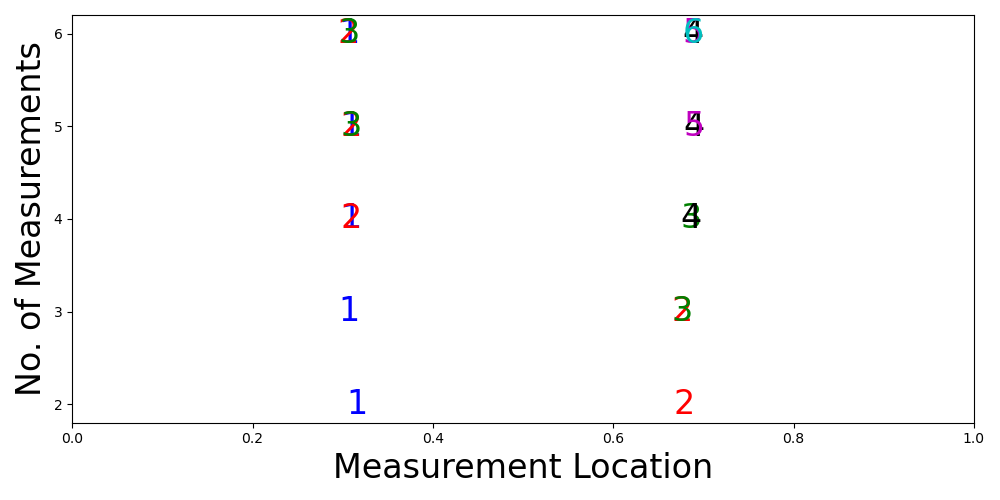
\includegraphics[height=0.5\textwidth]{dst_modelError0.png}
    \caption{Measurement clusterization for D-optimal designs for the
      inverse problem of the heat equation. Measurement locations were
      chosen according to the Bayesian D-optimality criterion of
      Theorem \ref{thm:d optimality}. Measurement locations are
      plotted over the computational domain \(\Omega = [0, 1]\)
      (x-axis), for varying numbers of measurements (y-axis). The
      colored numbers are measurement indices, plotted for visual
      clarity. Measurement clusterization already occurs for three
      measurements: the second measurement (red) is overlaid on the
      third (green). For five measurements, first (blue) and second
      (red) measurements are clustered, as well as the fourth (black)
      and the fifth (magenta).}
  \label{fig:clusterization illustration}
\end{figure}


Clusterization should not be confused with either repetition nor with
replication, which are commonly viewed as beneficial and even
necessary aspects of an optimal design \cite{fisher1949design,
  morris2011, schafer2001replication}. For example,
\cite{fisher1949design} in his famous milk and tea experiment,
suggested that repetition is a "way of enlarging the experiment and,
thereby, increasing its sensitiveness". In another example,
\cite{fay2000rainfall} measured the effect of rainfall on grass growth
in plots of land. The experiment involved fifteen "rainfall
manipulation shelters", where "Four rainfall manipulation treatments
(three replicates) then were assigned to 12 of the plots". While it
seems reasonable for the researchers to replicate the phenomenon they
are trying to study, clusterization is different: a clustered design
in the rainfall experiment would imply the researchers should take a
repeated measurement \emph{on the same plot}, at the expense of
measuring grass growth in other plots. In sharp contrast to repetition
and replication, clusterization is highly nonintuitive and we will see
that its origins run considerably deeper.


Researchers of inverse problems widely agree that measurement
clusterization is undesirable
\cite{fedorovDesignSpatialExperiments1996, nyberg2012, fedorov1997,
  Ucinski05, neitzel2019sparse}, prompting the exploration of various
remedies to address this issue. One approach involves merging close
measurements \cite{fedorov1997}; however, this strategy merely
overlooks the phenomenon of measurement clusterization. An alternative
solution lies in \emph{clusterization-free design}s, where measurement
locations are deliberately chosen to be distant from one another. This
can be achieved by imposing distance constraints between measurements
or by introducing correlated errors that account for both observation
error and model misspecification \cite{Ucinski05}. For instance, in
the context of time-series analysis for pharmacokinetic experiments,
measurement clusterization can be mitigated by incorporating the
modeling of auto-correlation time within the noise terms
\cite{nyberg2012}.


In spatial problems involving choice of measurements within a domain
\(\Omega \subseteq \mathbb{R}^d, d=1,2,3\), many researchers
circumvent the problem of measurement clusterization by choosing
measurements from a coarse grid in \(\Omega\) \cite{koval2020,
  alexanderian2021, attia2022, alexanderian2014, alexanderian2016,
  alexanderian2018efficient, brunton2016}. This approach incurs a
significant computational cost as it requires solving a difficult
combinatorial optimization problem for measurement locations over a
discrete set. The combinatorial optimization problem is usually
relaxed by first assigning optimal measurement weights in
\(\mathbb{R}_+\) to the potential measurement locations. Some
researchers incorporate a sparsifying \(\ell_1\) penalty term into the
design criterion, which is subsequently thresholded to achieve the
desired binary design over the coarse grid
\cite{horesh2008borehole}. Others progressively relax the \(\ell_1\)
penalty to an \(\ell_0\) penalty via a continuation method
\cite{alexanderian2016, alexanderian2014}. Others cast the problem of
finding optimal measurement weights as a stochastic optimization
problem \cite{attia2022stochastic}. All of the aforementioned methods
may indeed find a binary optimal design restricted to a given coarse
grid. However, none addresses one fundamental issue: the restriction
of measurement locations to a coarse grid in \(\Omega\) fundamentally
changes the optimal design problem and thus results in a sub-optimal
design.

Avoiding measurement clusterization is a pragmatic approach:
intuitively, researchers recognize that measurement clusterization is
undesirable, even though the underlying reasons may not be fully
clear. Consequently, they strive to prevent it and devise various
methodologies to avoid it. Yet each and every one of these
methodologies achieves its objective by imposing restrictions on
measurement locations, thereby fundamentally altering the optimal
design problem. To the best of my knowledge, no previous study has
tried to address some seemingly simple yet fundamental questions:
%
Why does imposing correlations between observations alleviate
measurement clusterization?
%
Is measurement clusterization a generic phenomenon? 
%
And, most importantly: Why does measurement clusterization occur?
%
%Should we aim to avoid measurement clusterization?
%
%Is it possible to substitute an optimal clustered design with an
%equally optimal non-clustered design?
%Can an optimal clustered design be relpaced with an equally optimal
%non-clustered design?


\subsection{Contribution}
The primary objective of this study is to provide a deep understanding
of measurement clusterization by addressing the aforementioned
questions. Our focus centers around investigating the Bayesian
D-optimality criterion. We conduct an analysis of Bayesian D-optimal
designs within the context of linear inverse problems over Hilbert
spaces and study two inverse problems: (a) In Sections
\ref{section:prelim} and \ref{section:D and grad} we propose a novel
relaxed model for an inverse problem where D-optimality maintains
analytical tractability, where D-optimal designs are identified via
Lagrange multipliers. This analytical framework facilitates the
exploration of the questions posed at the end of the previous
paragraph. We also study (b) the inverse problem of the 1D heat
equation from Section \ref{subsec:toy} above. Investigating both
inverse problems allows us to answer the questions posed in the
previous section:

\begin{enumerate}
\item \label{q:generic} \textbf{Is measurement clusterization a
  generic phenomenon?}
  %\subsection{An answer for Question \ref{q:generic}: Genericity of measurement clusterization}
  %% Computer implementation of Lemma \ref{thm:char} for the inverse
  %% problem outlined in Section \ref{section:how} also generates \(\obs\)
  %% as a solution to the D-optimal design problem.  Furthermore,
  We give two complementing answers to this question. First, from a
  theoretical perspective, we show that clusterization mainly depends
  on how quickly the eigenvalues of the prior measure in observation
  space decay. This decay depends mostly on how ill-posed the problem
  at hand is and does not depend much on the prior. See Section
  \ref{section:vanishing} --- particularly, Theorem \ref{thm:char} and
  the discussion following it. We also show results of numerical
  experiments, where simulations of our model give rise to D-optimal
  designs that exhibit clusterization with high probability in Section
  \ref{subsec:lemma sims}. Thus, given the genericity of our model, we
  expect measurement clusterization to be a generic and ubiquitous
  phenomenon.

\item \label{q:mitigate} \textbf{Why does imposing correlations
  between observations alleviate measurement clusterization?} In
  Section \ref{section:non vanishing}, we rigorously demonstrate the
  role of model error in mitigating clusterization, thereby
  corroborating earlier observations made by various
  researchers. Specifically, our proof shows that identical
  measurements result in no gain in design criterion when observation
  error tends to zero. Moreover, in Section \ref{subsec:corr errors
    sims}, we show that an error term corresponding to correlations
  between measurements mitigates clusterization in the inverse problem
  of the 1D heat equation.

\item \label{q:why} \textbf{Why does measurement clusterization
  occur?} In Section \ref{subsec:why} (specifically, See
  Fig~\ref{fig:why}) we give a compelling answer to this question by
  transporting insights we gain from our analytically tractable
  relaxed model to the inverse problem of the 1D heat equation. Our
  analysis reveals that a D-optimal design focuses on a select set of
  prior eigenvectors, specifically those with the largest eigenvalues
  in the prior covariance spectrum. In practical scenarios, the number
  of locations where (a) all relevant prior eigenvectors are
  significantly large, and (b) other eigenvectors are close to zero,
  is limited. Consequently, the clusterization of measurements arises
  as a natural consequence of the pigeonhole principle, as there are
  more measurements available than there are locations satisfying
  conditions (a) and (b).


  %% In Section \ref{section:vanishing}, we provide an insightful
  %% explanation for the optimality of clustered designs when no model
  %% error is present. We demonstrate that for our model, a D-optimal
  %% design measures only a small subset of prior eigenvectors, which are
  %% the prior eigenvectors with largest power spectrum. In real-life
  %% problems there are limited number of locations where: (a) the
  %% relevant prior eigenvectors are large, and other prior eigenvectors
  %% with large power in the prior spectrum are zero. Then measurement
  %% clusterization is a result of the pigeonhole principle, where there
  %% are more measurements than measurement locations satisfying (a) and
  %% (b).

  %% We conjecture that the prevalence of measurement clusterization
  %% arises due to the ease of discovering clustered designs.


%% \item \label{q:avoid} \textbf{Should we aim to avoid measurement
%%   clusterization?} Based on the analysis conducted in this study, we
%%   did not find any compelling reason to explicitly avoid optimal
%%   clustered designs.

%% \item \label{q:replace} \textbf{Is it possible to substitute an
%%   optimal clustered design with an equally optimal non-clustered
%%   design?} In Section \ref{section:vanishing}, we answer this question
%%   in the affirmative, although we show that numerical experiments
%%   conducted using our model indicate a strong preference for clustered
%%   designs.
\end{enumerate}

\subsubsection{Implications}
Our answer to Question \ref{q:generic} implies that encountering
clusterization should be expected in many different problems across
many different scientific fields. Thus, researchers that encounter
clusterization should not be surprised or wary. In Our answer to
Question \ref{q:why}, we explain what our view of the cause of
clusterization. As it appears, the cause is generic (see Question
\ref{q:why} above): a D-optimal design reduces uncertainty for a
select set of prior covariance eigenvectors --- those with the most
prior uncertainty, i.e.~those the practitioner cares about the most!
Consequently, practitioners should not try to avoid measurement
clusterization. Rather, practitioners should take repeated
measurements (e.g.~in MRI and borehole tomography), increase apparatus
sensitivity (e.g.~in EIT), or take consecutive measurements (e.g.~in
the 1D heat equation). Overall, we show that measurement
clusterization is a natural and (almost) inevitable part of Bayesian
D-optimal designs.

One interesting implication of the analysis presented here is that
clusterization can be expected once the number of measurements exceeds
the number of relevant eigenvectors. Since leading eigenvectors
typically correspond to slow variations in space and/or time,
clusterization could be used to estimate the number of relevant
degrees of freedom, and even to reduce the complexity of a
computational model, e.g.~by dropping discretization points.

It is important to note that we do not view measurement clusterization
as undesirable, nor do we believe it should be avoided at
all. Clusterization is a peculiar phenomenon and it is perfectly
reasonable for someone to argue against the D-optimality criterion
based on the fact that it results in clustered designs. We have seen,
however that there is perfectly reasonable explanation for
clusterization, i.e.~that clusterization arises when we seek a
designWe have shown that clusterization is an innevitable conseqeunce
of having a problem with modes of higher uncertainty than
others. Clusterization manifests the true underlying objective

Lastly, we believe that when clusterization arises, it should serve as
a warning sign to practitioners. In the inverse problem of the 1D heat
equation, clusterization occurs primarily because Laplacian
eigenvectors are nonzero almost everywhere in $\Omega$. Consequently,
measuring $u(x_1, T)$ at some point $x_1 \in \Omega$ provides
information about $u(x_2,T)$ for distant points $x_2 \in
\Omega$. Intuitively, this should not occur: for small $T$, the heat
distribution at $x_1$ should have minimal influence on the heat
distribution at $x_2$.

This behavior stems from a well-known property of the heat equation:
it allows information to spread instantly across the computational
domain \cite{renardy2006PDE}. In reality, heat and information
propagate at finite speeds. The emergence of clusterization in this
context is thus non-physical, arising from the nature of Laplacian
eigenvectors being nonzero almost everywhere. Clusterization therefore
indicates that the underlying mathematical model is overly permissive
and fails to capture crucial physical constraints. We suggest that
when clusterization occurs, practitioners should consider alternative
models where information is localized in space and travels at finite
speeds. Such models may not only provide more physically accurate and
meaningful results but may also mitigate the issue of clusterization.



\subsubsection{Other Contributions}
In Theorem \ref{thm:char}, we also show that D-optimal designs are
best understood in the sapce of \emph{observations}, see Section
\ref{section:vanishing} for a precise statement. This is in accordance
with previous work by \cite{koval2020}, who showed that A-optimal
designs are best constructed in the space of observations.

In the process of proving Theorem \ref{thm:char} we prove and
generalize several lemmas. Among those, is Lemma \ref{lemma:free},
which is (to the the best of my knowledge) novel: We decompose a
symmetric positive definite matrix \(M \in \mathbb{R}^{k \times k}\)
with \(\ttr M = m \in \mathbb{N}\) as \(M = AA^t\), where \(A\in
\mathbb{R}^{k \times m}\) has unit norm columns.

%% Finally, in Lemma \ref{lemma:lax} we generalize a lemma for
%% calculating \(\frac{\der}{\der t} \log \det (I + X(t))\), where
%% \(X(t)\)is an operator valued function \cite{Lax07}.

%% Finally, we must stress that we do not advocate any particular
%% solution to clusterization. We do not suggest that clustered designs
%% should be abandoned, nor do we support the use of clustered designs in
%% any circumstances. Our goal is to investigate an intriguing phenomenon
%% of clusterization and seek a deeper understanding for it. Different
%% researchers in different disciplines have differenot viewed as a problem. For
%% example, \cite{lozan} suggest in the introduction section that
%% repeated measurements are necessary. Our results align with that
%% common wisdom and settle the seemed contradiction.


\subsection{Limitations}\label{subsec:limitations}
The main limitation of this study is that our generic model does not
correspond to any specific real-life problem. Specifically, in its
current form, our model does not allow point evaluations. Thus, while
our model is generic enough to be analytically tractable, some may
argue that our model is too far removed from any real application. To
these claims I would answer that scientists have a long history of
studying models that are bare-bones simplifications of real systems,
e.g.~the Ising model \cite{cipra1987}, the Lorenz system \cite{brin},
the Lotka-Volterra equations \cite{logan2006}, the Carnot engine
\cite{kardar2007} and many others.
\section{Preliminaries and Notation}\label{section:prelim}
Here we present the basics of Bayesian inverse problems over hilbert
spaces. Since we are ultimately interested in inferring a function
over some domain, we will keep in mind that these Hilbert spaces
should really be thought of as function spaces. A deeper treatment of
the foundations for inverse problems over function spaces can be found
in \cite{Stuart10}.


\subsection{Forward Problems}\label{subsec:abstract OED}
In this section we give definitions and notations for forward problems,
which are an essential part of the inverse problems we discuss
later. Consider a "parameter space" \(\hilp\) and an "observation
space" \(\hilo\) --- both separable Hilbert spaces (the subscripts p
and o are for "parameter" and "observation", respectively). The
parameter space includes the quantity we seek to infer; in the inverse
problem of the heat equation, the parameter space $\hilp$ is where the
initial condition lives. The observation space $\hilo$, on the other
hand, is the space from which we take measurements; in the example of
the 1D heat equation, $u(\cdot, T) \in \hilo$.

The connection between parameter and observation spaces is made by the
\emph{forward operator} \(\fwd: \hilp \to \hilo\). We assume the
forward operator \(\fwd\) is linear. In the inverse problem of the 1D
heat, the forward operator is determined by the time evolution of the
1D heat equation \eqref{eq:heat1} and \eqref{eq:heat2}.

Measurements are taken via a \emph{measurement operator} \(\obs\). It
is common for the measurement and forward operators to be merged
\(\tmp := \obs \fwd\) \cite{AlexanderianGloorGhattas14}, but the
analysis carried out in the following sections requires that \(\fwd\)
and \(\obs\) are explicitly separated (as in
\cite{attia2022stochastic, cvetkovic2023choosing}). Note that \(\obs
\in ( \hilo^* )^m\), where \(m\) is the number of measurements
taken\footnote{The alert reader will likely ask how do we reconcile
point measurements $\delta_x$ as suggested by the formulation of the
1D heat equation with workin in Hilbert spaces. We don't. This entire
study could be formulated for Banach spaces where point measurements
are allowed. We avoid this technical difficulty because: (1) it does
not add much to the study, (2) it is beyond the technical abilities of
the author}. Entries \(\meas_j, j=1,\dots,m\) of the measurement
operator \(\obs\) are called \emph{measurements}:

\begin{equation*}%\label{eq:O}
  \obs u = (\meas_1(u), \dots, \meas_m(u) )^t \in \R^m,\ u \in \hilo.
\end{equation*}

Data is acquired via noisy observations, and we consider two types of
error terms: Spatially correlated model error \(\eps' \sim
\normal(0,\modcov)\) with \(\modcov\) a covariance operator; and
observation error denoted \(\eps \sim \normal(0, \sigma^2 I_m)\), with
\(I_m \in \mathbb{R}^{m \times m}\) the identity. Both error terms and
the prior (see below) are assumed independent of each other. Thus,
data is acquired via
\begin{align}\label{eq:inverse problem}
  \data := \obs (\fwd \param + \eps') + \eps = \obs \fwd \param + \obs \eps' + \eps.
\end{align}

It is easy to verify that \(\obs \eps' + \eps \in \R^m\) is a centered
Gaussian random vector with covariance matrix

\begin{align}\label{eq:Sigma}
  \begin{split}
    \Sigma(\obs) :&= \mathbb{E}[ (\obs \eps' + \eps) (\obs \eps' +
      \eps)^t ]
    % 
    % 
    = \obs \modcov \obs^* + \sigma^2I_m , 
  \end{split}
\end{align}
where
\begin{align}\label{eq:modcov explained}
  \begin{split}
    [\obs \modcov \obs^*]_{ij} & = e_i^t \obs \modcov \obs^* e_j 
    %
    %
    %
    = \meas_i (\modcov \meas_j).% \text{ (by \eqref{eq:obs*})}.
  \end{split}
\end{align}
Taking \(\modcov = 0\) is a common practice
\cite{tarantola2005,kaipio2005,Vogel02} and then \(\Sigma =
\sigma^2I_m\) is a scalar matrix which does not depend on \(\obs\).

\subsection{Bayesian Linear Inverse Problems}\label{subsec:bayesian inverse problems}
In the previous section, we saw how a parameter $u\in \hilp$ is
transported to the observation space via the forward operaror $\fwd u
\in \hilo$, how observations are generated from a parameter via $\obs
\fwd u$ and how observations and noise give rise to data $\data$. It
is time to formulate the process of inferring the parameter as a
Bayesian inverse problem. The first ingredient we need is a prior.

We take a Gaussian prior \(\param \sim \pr = \normal(\prmean
,\prcov)\) with some appropriate covariance operator \(\prcov\) on
\(\hilp\) \cite{Stuart10}. For example, for the inverse problem of the
1D heat equation we chose $\prcov = -\Delta^{-1}$ --- see Section
\ref{subsec:toy}. Note that \(\fwd \prcov \fwd^*\) is the prior
covariance in \(\hilo\) \cite{Stuart10}, and as such is assumed
invertible --- an assumption which we will use later (if \(\fwd\) has
a nontrivial kernel we utilize Occam's Razor and ignore said kernel
altogether).

Since $\fwd$ is linear and $\pr$ is Gaussian --- the posterior
\(\post\) is Gaussian as well. We do not utilize the posterior mean in
this study, but the posterior covariance operator $\postcov$ is given
by the known formula\cite{Stuart10}:
\begin{align}\label{eq:postcov}
  \postcov = (\prcov^{-1} + \fwd^* \obs^* \Sigma^{-1} \obs \fwd
  )^{-1}.
\end{align}

\subsection{Bayesian D-Optimal Designs}\label{subsec:D optimal design} 
A Bayesian D-optimal design maximizes the expected KL divergence
between posterior \(\post\) and prior measures \(\pr\). For arbitrary
posterior and prior measures, the KL divergence is defined,
analogously to eq.~\ref{eq:basic KL}, via the Radon-Nikodym
derivative:
\begin{equation*}
  D_{KL}(\post||\pr) = \int \log \frac{\der \post}{\der \pr}(\param) \der \post(\param).
\end{equation*}

The study of D-optimal designs for Bayesian linear inverse problems in
infinite dimensions was pioneered by \cite{AlexanderianGloorGhattas14,
  alexanderian2018efficient}. The main result we will make use of is
summarized (in our notation) below:

\begin{theorem}[Alexanderian, Gloor, Ghattas \cite{AlexanderianGloorGhattas14}]\label{thm:d optimality}
  Let \(\pr = \normal(\prmean,\prcov)\) be a Gaussian prior on \(\hilp\)
  and let \(\post = \normal(\postmean,\postcov)\) the posterior measure
  on \(\hilp\) for the Bayesian linear inverse problem \(\data = \obs
  \fwd\param + \obs \eps' + \eps\) discussed above. Then
  \begin{align}\label{eq:objective}
    \begin{split}
      \tar( \obs) :&= \mathbb{E}_{\data}\left [ D_{\text{KL}} (\post || \pr ) \right ] \\
      % 
      % 
      % 
      &= \frac12 \log \det 
      ( I + \prcov^{1/2}  \fwd ^* \obs^* \Sigma^{-1} \obs \fwd \prcov^{1/2}).
    \end{split}
  \end{align}
\end{theorem}

Note that in \cite{AlexanderianGloorGhattas14,
  alexanderian2018efficient}, results are stated for \(\Sigma=I\)
(implied by \(\modcov = 0,\sigma^2=1\)), but these results also hold
for more general covariance matrices
\cite[p. 681]{AlexanderianGloorGhattas14}.

%% It is important to note that since \(\obs\) is finite-rank,
%% \(\prcov^{1/2} \fwd ^* \obs^* \Sigma^{-1} \obs \fwd \prcov^{1/2}\) is
%% trace-class.
\begin{definition}\label{def:d optimality}
  We say \(\opt\) is \emph{D-optimal} if \(\opt =
  \argmax_{\obs} \tar(\obs)\), where entries of \(\obs \in (\hilo^*)^m\)
  are constrained to some allowed set of measurements in \(\hilo^*\).
\end{definition}

Intuition for Theorem \ref{thm:d optimality} can be gained by
recalling from Section \ref{subsec:D} that for a Bayesian linear model
in finite dimensions, with Gaussian prior and Gaussian noise, a
D-optimal design minimizes the determinant of the posterior covariance
matrix. Theorem
\ref{thm:d optimality} and Definition \ref{def:d optimality} carry a
similar intuition:
\begin{align*}
  \begin{split}
    \tar(\obs) &= \frac12 \log \det ( I + \prcov^{1/2}  \fwd ^* \obs^* \Sigma^{-1} \obs \fwd \prcov^{1/2}) \text{ by \eqref{eq:objective}}\\
    &= \frac12 \log \det \Big( \prcov ( \prcov^{-1} + \fwd ^* \obs^* \Sigma^{-1} \obs \fwd) \Big )\\
    &= \frac12 \log \det \prcov \postcov^{-1} \text{ by \eqref{eq:postcov}}.
    %%  &= \frac12 \log \det \prcov -\frac12 \log \det \postcov.
  \end{split}
\end{align*}
We think of \(\prcov\) as constant, in the sense that $\prcov$ does
not depend on data $\data$. Thus, a D-optimal design minimizes a
quantity analogous to the posterior covariance determinant, similarly
to the finite-dimensional case.


%% \subsection{Notation Summary}\label{subsec:notation}
%%   Our notation is summarized below. We let:
%%   \begin{itemize}
%%   \item \(\hilp, \hilo\) Hilbert spaces.
%%   \item \(\fwd:\hilp \to \hilo\) a linear compact operator.
%%   \item \(\pr \sim \mathcal{N}(0, \prcov)\) prior Gaussian measure on
%%     \(\hilp$, with prior covariance operator \(\prcov:\hilp \to \hilp$.
%%   \item \(\obs: \hilo \to \mathbb{R}^m\) measurement operator, where \(m
%%     \in \mathbb{N}\) is the number of measurements taken.
%%   \item \(\sigma^2 \in \mathbb{R}_{+}\) observation noise variance.
%%   \item \(\modcov\) model error covariance operator.
%%     %% \(\data = \obs \fwd \param + \eps$, where \(\eps \in
%%     %% \mathbb{R}^m\) isiid \(\mathcal{N}(0, \sigma^2)\) noise.
%%   \item \(\Sigma(\obs) = \obs \modcov \obs^* + \sigma^2I$. 
%%   \item \(\post\) the posterior measure, with covariance \(\postcov$.
%%   \item A D-optimality design criterion
%%     \cite{AlexanderianGloorGhattas14}:
%%     \begin{align*}
%%       \begin{split}
%%         \tar(\obs) :&= \mathbb{E}_{\data}\left [ D_{\text{KL}} (\post || \pr ) \right ] \\
%%         % 
%%         % 
%%         % 
%%         &= \frac12 \log \det ( I + \prcov^{1/2} \fwd ^* \obs^* \Sigma(\obs)^{-1} \obs
%%         \fwd \prcov^{1/2}).
%%       \end{split}
%%     \end{align*}
%%   %% \item \(\{\lambda_i\}_{i=1}^\infty\) eigenvalues of \(\fwd\prcov\fwd^*$
%%   %%   in decreasing order of magnitude.
%%   %% %% \item \(\{\ev_i\}_{i=1}^\infty\) their corresponding eigenvectors.
%%   %% \item \(\{\eta_i\}_{i=1}^\infty\) eigenvalues of \(\obs^*\obs$.
%%   \end{itemize}


%% \subsection{Sequential vs Simultaneous Optimization}\label{subsec:seq vs sim}
%% From defintion \ref{def:d optimality} we wish to characterize solution(s) of the
%% following optimization problem for \(\tar$. %%: (\hilo^*)^m \to \R$:
%% \begin{align}\label{eq:optimization}
%%   \obs^{\star} := \argmax_{\obs} \tar( \obs ) 
%%   = \argmax_{\obs} \frac12 \log \det 
%%   (I + \prcov^{1/2} \fwd^*\obs^* \Sigma^{-1} \obs \fwd \prcov^{1/2}),
%% \end{align}
%% where \(\obs\) is constrained to some allowed set of observations. We
%% call this problem ``simultaneous optimization'', since all
%% observations are decided on simulatneously.

%% For computational reasons, one may prefer to find the best
%% observations in a sequential manner. Denote
%% \begin{equation}\label{eq:def obs_k}
%%   \obs_k := (\meas_1,\dots, \meas_k)^t,  k\leq m.
%% \end{equation}
%% Sequential optimal design proceeds as follows. Find \(\meas_1\) by
%% maximizing \(\tar(\obs_1)$. Then, keeping \(\meas_1\) fixed --- find
%% \(\meas_2\) as the maximizer of \(\tar(\obs_2)$. Then, find \(\meas_3\) by
%% keeping \(\meas_1,\meas_2\) fixed and taking \(\meas_3\) as the maximizer
%% of \(\tar(\obs_3)$. Continue this way until \(\obs_m = \obs\) is
%% found, where \(m\) is the number of available observations. %% It is
%% %% important to notice that this scheme does not require actually
%% %% observing data --- in \eqref{eq:objective} data is averaged out.

%% The analysis in this paper is conducted for the general simultaneous
%% optimization case. The sequential optimization case is dealt with in
%% section \ref{subsec:clusterization sequential}. It is important to
%% note, however that all conclusions we arrive at for the simultaneous
%% case easily specialize to the sequential case by considering the
%% posterior as the next sequential step's prior.

\section{The Constrained Optimization Problem of D-Optimal Design}\label{section:D and grad}
We seek a formulation of the D-optimal design problem via Lagrange
multipliers. We first find the gradient of $\tar$, then we suggest
unit-norm constraints on $\obs$ and find their gradients. Results of
this section are summarized in Theorem \ref{thm:constrained}. First,
recall that:
\begin{definition}\label{def:var}
  Let $F$ a real valued function of $\obs$. The first variation of $F$
  at $\obs$ in the direction $V$ is:
  \begin{equation*}
    \delta F(\obs) V := \frac{\der}{\der \tau}\Big |_{\tau=0}  F( \obs + \tau V).
  \end{equation*}

  Moreover, if
  \begin{equation*}
    \delta F(\obs) V = \tr{\nabla F(\obs) V},
  \end{equation*}
  then we call $\nabla F(\obs)$ the gradient of $F$ at $\obs$. 
\end{definition}

%% Gradients are best thought of as row vectors. This will prove
%% important in section \ref{subsec:necessary}.


%% \subsection{The gradient of $\tar$}\label{section:objective}

\begin{proposition}\label{prop:tar grad}
  The gradient of the D-optimality objective $\tar$ is
  \begin{equation*}
    %% \delta \tar(\obs) V = \tr{V ( I - \modcov \obs^* \Sigma^{-1}\obs )
    %%   \fwd \postcov \fwd^* \obs^* \Sigma^{-1}}.
    \nabla \tar(\obs) = ( I - \modcov \obs^* \Sigma^{-1}\obs ) \fwd
    \postcov \fwd^* \obs^* \Sigma^{-1}
  \end{equation*}
\end{proposition}

The proof amounts to calculating the variational derivative of $\tar$
at $\obs$ for any direction $V$ (by Definition \ref{def:var}) and is
delegated to the Supplementary.


\subsection{Unit norm constraints and their gradient}
In a real-life optimal design problem we cannot choose any measurement
operator $\obs \in (\hilo^*)^m$. In order to facilitate analysis, we
seek reasonable constraints on $\obs$ for which finding a D-optimal
design is analytically tractable. The following proposition will guide
us in finding such constraints.

\begin{proposition}\label{prop:bigger better}
  Let $\obs = (\meas_1,\dots,\meas_m)^t$, $j \in \{1,\dots,m\}$,
  $\sigma^2 > 0$ and $|\zeta| > 1$. Then $\tar(\obs)$ increases if we
  use $\zeta \meas_j$ in $\obs$ instead of $\meas_j$.
\end{proposition}

\begin{proof} 
  Fix $j=1,\dots,m$ and take $V:= e_j e_j^t \obs$. For $u
  \in \hilo$:
  \begin{equation*}
    Vu = e_je_j^t (\meas_1(u),\dots,\meas_m(u) )^t = e_j \meas_j(u)
    = (0,\dots,0,\meas_j(u),0,\dots,0)^t.
  \end{equation*}
  %% This way, $V$ has the same $j$th entry as $\obs$ while the rest
  %% are set to zero.
  We now calculate the variation of $\tar$ at $\obs$ in the direction
  of $V$. Denote $\tmp: = \fwd \postcov \fwd^*$. From Proposition
  \ref{prop:tar grad}:
  \begin{align*}
     \delta \tar(\obs) V 
    &= \tr{V ( I - \modcov \obs^*\Sigma^{-1}\obs) \tmp \obs^* \Sigma^{-1}} \\
    % 
    %
    %
    &= \tr{e_je_j^t \obs ( I - \modcov \obs^*\Sigma^{-1}\obs) \tmp \obs^* \Sigma^{-1}} \\
    %
    % 
    %
    &= e_j^t \obs ( I - \modcov \obs^*\Sigma^{-1}\obs) \tmp \obs^* \Sigma^{-1}e_j \\
    %
    % 
    %
    &= e_j^t ( I - \obs \modcov \obs^*\Sigma^{-1})\obs \tmp \obs^* \Sigma^{-1}e_j \\  
    % 
    %
    %
    &=  e_j^t(\Sigma-\obs \modcov \obs^*) \Sigma^{-1}\obs \tmp \obs^* \Sigma^{-1}e_j \\
    %
    %
    %
    &=\sigma^2 e_j^t \Sigma^{-1}\obs \tmp \obs^* \Sigma^{-1}e_j
    \text{ by \eqref{eq:Sigma} }\\
    %
    % 
    %
    &=\sigma^2 e_j^t \Sigma^{-1}\obs \fwd \postcov \fwd^* \obs^* \Sigma^{-1}e_j.
  \end{align*} 
  Since $\postcov$ is positive definite, we conclude that $\delta
  \tar(\obs) V > 0$. This means that increasing the magnitude of the
  $j^{\text{th}}$ measurement functional increases $\tar(\obs)$.
\end{proof}

Proposition \ref{prop:bigger better} implies that it is a good idea to
bound the norm of measurements. If, for example, we can take
measurements in $\textup{span}\{\meas\}$ for some $\meas \neq 0$, then
the the D-optimality criterion is unbounded. In contrast, in any
real-life problem where sensors are concerned, the norm of
measurements recorded by sensors is always one\footnote{Again, our
analysis does not apply to point evaluations. These are just used for
motivation and can be approximated by elements in $\hilo^*$ as long as
$\hilo$ is a function space, e.g.~$L^2(\Omega)$.}:

\begin{equation}
  \| \delta_{\x} \| = \sup_{0 \neq u \in C(\Omega)}
  \frac{
    |\int_{\Omega}u(\y) \delta_{\x}(\y) \der \y|
  }{
    \sup|u|
  } = \sup_{0 \neq u \in C(\Omega)} \frac{|u(\x)|}{\sup|u|} = 1,
  \forall \x \in \Omega.
\end{equation}

Thus, it is reasonable to consider measurements with unit $\hilo^*$
norm. We can write the unit norm constraints as a series of $m$
equality constraints (one for each measurement) on $\obs$. We define
them and find their gradients in Proposition \ref{prop:constraints
  grad} below, whose proof is straightforward and delegated to the
Supplementary:

\begin{proposition}\label{prop:constraints grad}
  Let
  \begin{align*}
    \phi_j(\obs) :=\frac12 \| \obs^* e_j\|_{\hilp}^2 - \frac12 = 0,\ j=1,\dots,m.
  \end{align*}
  Then
  \begin{equation*}
    %% \delta \phi_j(\obs)V = \tr{V \obs^* e_je_j^t}.
    \nabla \phi_j(\obs) = \obs^* e_je_j^t.
  \end{equation*}
\end{proposition}

%% The same arguments justifying \eqref{eq:tar grad} hold here, and thus:

%% \begin{align}\label{eq:grad constraints}
%% \nabla \phi_j(\obs) = \obs^* e_j e_j^t = \meas_j e_j^t , j=1,\dots,m,
%% \end{align}
%% where $\nabla \phi_j(\obs) \in \hilo^m$. As noted at the end of
%% Section \ref{section:objective},

%% The gradients $\nabla \tar(\obs)$ and $\nabla \phi_j(\obs)$ are best
%% thought of as row vectors.

\subsection{Necessary conditions for D-optimality}
We find necessary first-order conditions for D-optimality via Lagrange
multipliers:

\begin{align}
  &\nabla \tar(\obs) = \sum_{j=1}^m \xi_j \nabla \phi_j (\obs)
  \label{eq:Lagrange mult1} \\
    &\phi_j(\obs) = 0, j = 1,\dots,m. \label{eq:Lagrange mult2}
\end{align}

We now substitute the gradients calculated in Propositions
\ref{prop:tar grad} and \ref{prop:constraints grad} into
\eqref{eq:Lagrange mult1}:
\begin{equation}\label{eq:constrained}
  (I - \modcov \obs^* \Sigma^{-1} \obs) \fwd \postcov \fwd^* \obs^*\Sigma^{-1}
  = \sum_{j=1}^m \xi_j \obs^* e_je_j^t = (\xi_1 \meas_1,\dots,\xi_m \meas_m).
\end{equation} 
Letting $\Xi := \diag(\xi_j)$, we can write \eqref{eq:constrained} and
\eqref{eq:Lagrange mult2} more compactly as:

\begin{theorem}[Necessary conditions for D-Optimality]\label{thm:constrained}
  Let:
  \begin{equation*}
    \opt = \argmax_{\|\meas_j\| = 1, j=1,\dots,m}\tar(\obs).
  \end{equation*}
  
  Then:
  \begin{equation*}
    ( I - \modcov \opt^* \Sigma^{-1} \opt) \fwd \postcov \fwd^* \opt^*  \Sigma^{-1}
    = \opt^* \Xi, 
  \end{equation*}
  where $\Xi \in \mathbb{R}^{m \times m}$ is diagonal.
\end{theorem}




%% Imposing correlations between observations alleviate measurement clusterization
\section{Answer to Question \ref{q:mitigate}: Model error mitigates clusterization}\label{section:non vanishing}
We now show that if $\modcov \neq 0$ clusterization will not occur. It
is known that including a model error term mitigates the
clusterization phenomenon \cite{Ucinski05}, and here we prove this
rigorously. Let $\obs = (\meas_1,\dots,\meas_m)^t$ and $\obsm :=
(\meas_1,\dots,\meas_{m-1})^t$. Denote $\Sigmam := \Sigma (\obsm)$ and
$\postcovm$ the posterior covariance that arises when $\obsm$ is
utilized as a measurement operator.

\begin{proposition}[Increase due to a measurement]\label{prop:design increase}
  Let $\obs = (\meas_1,\dots,\meas_m)^t$ and $\obsm :=
  (\meas_1,\dots,\meas_{m-1})^t$. Then
  \begin{equation}\label{eq:conclusion}
    \tar( \obs ) - \tar (\obsm ) =
    \frac12 \log \left ( 1 + \frac{
      \langle \fwd \postcovm \fwd^* (\obsm^* \Sigmam^{-1} \modcov - I ) \meas_m,
      (\obsm^* \Sigmam^{-1} \modcov - I ) \meas_m \rangle
    }{
      \sigma^2 + \meas_m \modcov \meas_m - \meas_m \modcov \obsm^* \Sigmam^{-1} \obsm \modcov \meas_m 
    }       
    \right ).
  \end{equation}
\end{proposition}
The proof is long and tedious, and is delegated to the Supplementary.


\begin{corollary}\label{cor:same meas}
  If $\meas_m = \meas_j$ for some $1 \leq j \leq m-1$, then
  \begin{equation*}
    \tar(\obs) - \tar(\obsm) =
    \log \left ( 1 + \frac{\sigma^2
      \langle \fwd \postcovm \fwd^* \obsm^* \Sigmam^{-1} e_j,
      \obsm^* \Sigmam^{-1}e_j \rangle
    }{
      2 - \sigma^2 e_j^t\Sigmam^{-1}e_j 
    }       
    \right ),
  \end{equation*}
  where $e_j\in \mathbb{R}^{m-1}$ is the $j^{\text{th}}$ standard unit
  vector.
\end{corollary}

\begin{proof} \label{cor:same meas proof}
  Denote $A:= \obs \modcov \obs^*$ and $v_j$ the $j^{\text{th}}$
  column of $A$.  Note that $v_j = \obsm \modcov \meas_m$, since
  $(\obsm \modcov \obsm^*)_{ij} = \meas_i(\modcov \meas_j)$, as
  explained in \eqref{eq:modcov explained}. We can now verify that
  \begin{equation}\label{eq:observation}
    \Sigmam^{-1} \obsm \modcov \meas_m = \Sigmam^{-1}v_j = (A +\sigma^2I_{m-1})^{-1} v_j =
    e_j -\sigma^2 \Sigmam^{-1}e_j.
  \end{equation}
  %
  Using \eqref{eq:observation}:
  \begin{align}\label{eq:denominator}
    \begin{split}
      \meas_m \modcov \obsm^* \Sigmam^{-1} \obsm \modcov \meas_m
      &= \meas_m \modcov \obsm^* ( e_j - \sigma^2 \Sigmam^{-1} e_j )\\
      %
      %
      %
      &= \meas_m \modcov \meas_j - \sigma^2 \meas_m \modcov \obsm^* \Sigmam^{-1}e_j \\
      %
      %
      %
      &= \meas_m \modcov \meas_j -\sigma^2 (e_j - \sigma^2 \Sigmam^{-1}e_j)^t e_j \\
      %
      %
      %
      &= \meas_m \modcov \meas_m -\sigma^2 + \sigma^4 e_j^t\Sigmam^{-1}e_j.
    \end{split}
  \end{align}
  We use \eqref{eq:observation} to simplify the enumerator in
  \eqref{eq:conclusion}:
  \begin{align}\label{eq:enumerator}
    \begin{split}
      (\obsm^* \Sigmam^{-1} \obsm \modcov - I ) \meas_m
      &= \obsm^* \Sigmam^{-1} \obsm \modcov \meas_m - \meas_m \\
      %
      %
      %
      &= \obsm^* (e_j - \sigma^2 \Sigmam^{-1} e_j) -\meas_j \\ 
      %
      %
      %
      &= -\sigma^2 \obsm^* \Sigma^{-1}e_j. 
    \end{split}
  \end{align}
  %
  Now, we substitute \eqref{eq:enumerator} and \eqref{eq:denominator}
  to the enumerator and denominator of \eqref{eq:conclusion}:
  %
  \begin{align*}
    \tar( \obs ) - \tar (\obsm ) &=
    \log \left ( 1 + \frac{
      \langle \fwd \postcovm \fwd^* (\obsm^* \Sigmam^{-1} \modcov - I ) \meas_m,
      (\obsm^* \Sigmam^{-1} \modcov - I ) \meas_m \rangle
    }{
      \sigma^2 + \meas_m \modcov \meas_m - \meas_m \modcov \obsm^* \Sigmam^{-1} \obsm \modcov \meas_m 
    }       
    \right ) \\
    %
    %
    %
    &= \log \left ( 1 + \frac{\sigma^4
      \langle \fwd \postcovm \fwd^* \obsm^* \Sigmam^{-1} e_j,
      \obsm^* \Sigmam^{-1}e_j \rangle
    }{
      2\sigma^2 - \sigma^4 e_j^t\Sigmam^{-1}e_j 
    }       
    \right ) \\
    %
    %
    %
    &= \log \left ( 1 + \frac{\sigma^2
      \langle \fwd \postcovm \fwd^* \obsm^* \Sigmam^{-1} e_j,
      \obsm^* \Sigmam^{-1}e_j \rangle
    }{
      2 - \sigma^2 e_j^t\Sigmam^{-1}e_j 
    }       
    \right ).
  \end{align*}
\end{proof}


Recall from \eqref{eq:Sigma} that $\Sigma(\obs) = \obs
\modcov \obs^* + \sigma^2I$ and let $u := \obsm^*
\Sigmam^{-1}e_j$. Then

\begin{align*}
  \begin{split}
    \lim_{\sigma^2 \to 0} u &= \obsm^*(\obsm \modcov \obsm^*)^{-1}e_j\\
    \lim_{\sigma^2 \to 0} \postcovm &= (\prcov^{-1} + \fwd^* \obsm^* (\obsm \modcov \obsm^*)^{-1} \obsm \fwd)^{-1} \text{ (From \eqref{eq:postcov})}.
  \end{split}
\end{align*}

Consequently, 
\begin{equation*}
   \langle \fwd \postcovm \fwd^* \obsm^* \Sigmam^{-1}
    e_j, \obsm^* \Sigmam^{-1}e_j \rangle 
  %
  %
  = \langle \fwd \postcovm \fwd^* u, u \rangle
\end{equation*}

is bounded, and

\begin{equation*}
\lim_{\sigma^2 \to 0} \tar(\obs) -\tar(\obsm) = 0.
\end{equation*}

We have shown that in the limit $\sigma^2 \to 0$, no increase in
$\tar$ is achieved by repeating a measurement. Thus, for vanishing
noise levels, clustered designs cannot be D-optimal. For repeated
measurements and $\sigma^2=0$, $\Sigma$ is not invertible and the
posterior covariance is not defined in eq.~\eqref{eq:postcov}. We can
\emph{define} the posterior in this case to equal the posterior when
the repeated measurement is dropped, and under this definition, a
repeated measurement trivially does not increase the design criterion
when $\sigma^2=0$. Our results are stronger, since we show
\emph{continuity} in $\sigma^2$.

It is worth noting that by the nonnegativity of the KL divergence,
$\tar$ cannot decrease upon adding measuremnts. However, we can
construct examples where the posterior is not changed upon taking a
new measurement e.g.~if the prior variance vanishes on some
eigenvector and a measuremnt is taken on said eigenvector. We do not
expect a measurement to generate no information whatsoever in any
realistic scenario, and we choose to ignore such pathologies.

In conclusion, for small observation error $\sigma^2$ levels,
measurement clusterization is mitigated by the presence of a non-zero
model error $\modcov$ --- answering Question \ref{q:mitigate} posed in
the Introduction.% Section \ref{section:intro}.
\section{D-Optimal Designs Without Model Error}\label{section:vanishing}
Our goal in this section is to prove Theorem \ref{thm:char} which
characterizes D-optimal designs when $\modcov = 0$. The necessary
first-order condition for D-optimality of Theorem
\ref{thm:constrained} for $\modcov = 0$ become:

\begin{equation}\label{eq:eigenproblem}
  \sigma^{-2}\fwd \postcov \fwd^* \obs^* = \obs^* \Xi,
\end{equation}
with $\Xi$ diagonal. Equation \eqref{eq:eigenproblem} looks like an
eigenvalue problem for the self-adjoint operator $\sigma^{-2}\fwd
\postcov \fwd^*$, where rows of $\obs$, namely $\meas_j,j=1,\dots, m$,
are eigenvectors. However, $\postcov$ depends on $\obs$, so we refer
to \eqref{eq:eigenproblem} as a \emph{nonlinear} eigenvalue problem.
%% Proposition \ref{prop:twice woodbury} and Lemma \ref{lemma:sim
%% diag} required

\begin{proposition}\label{prop:twice woodbury}
  Assume $\fwd \prcov \fwd^*$ is invertible. Then
  \begin{align*}
    \begin{split}
      \fwd( \prcov^{-1} + \sigma^{-2}  \fwd^* \obs^* \obs \fwd )^{-1} \fwd^* 
      %
      %
      = \left ( (\fwd\prcov\fwd^*)^{-1} + \sigma^{-2}  \obs^* \obs \right )^{-1},
    \end{split}
  \end{align*}  
\end{proposition}

As we mentioned in Section \ref{subsec:bayesian inverse problems},
$\fwd \prcov \fwd^*$ is the prior covariance $\hilo$ and could be
safely assumed invertible. The proof of Proposition \ref{prop:twice
  woodbury} is delegated to the Supplementary. It amounts to using
Woodbury's matrix identity twice. The standard proof for Woodbury's
matrix identity works for separable Hilbert spaces, as long as all
terms are well defined. Unfortunately, $\obs^*\obs$ is not invertible,
so we utilize a regularization trick to force it to be.

\begin{lemma}[Simultaneous diagonizability]\label{lemma:sim diag}
  Let $\hil$ separable Hilbert space, $C:\hil \to \hil$ self-adjoint
  and $\func_1,\dots,\func_m \in \hil$. Denote $\func^*$ the element
  $\func$ acting as a linear functional. If
  \begin{equation*}
   (C + \sum_{j=1}^m \func_j\func_j^*) \func_l = \xi_l \func_l,\ l = 1,\dots,m
  \end{equation*}
  then $C$ and $\sum_{j=1}^m \func_j \func_j^*$ are simultaneously
  diagonalizable.
\end{lemma}
The proof of Lemma \ref{lemma:sim diag} is delegated to the
Supplementary.

\begin{proposition}\label{prop:same ev}
  Let $\obs$ satisfy the nonlinear eigenvalue problem
  \eqref{eq:eigenproblem}. Then $\obs^*\obs$ and $\fwd \prcov \fwd^*$
  are simultaneously diagonalizable.
\end{proposition}
\begin{proof}
  \begin{align}\label{eq:mod conditions}
    \begin{split}
      \obs^* \Xi &= \sigma^{-2}\fwd \postcov \fwd^* \obs^*  \text{ (by \eqref{eq:eigenproblem})}\\
      %
      %
      %
      &= \sigma^{-2} \fwd( \prcov^{-1} + \sigma^{-2}  \fwd^* \obs^* \obs \fwd )^{-1} \fwd^* \obs^*  \text{ (by \eqref{eq:postcov})} \\
      %
      %
      %
      &= \sigma^{-2} \left ( (\fwd\prcov\fwd^*)^{-1} + \sigma^{-2}  \obs^* \obs \right )^{-1} \obs^* \text{ (by Proposition \ref{prop:twice woodbury})}.
    \end{split}
  \end{align}

  Now take $\func_j^{*} = \meas_j$ and $C := (\fwd \prcov
  \fwd^*)^{-1}$ and use Lemma \ref{lemma:sim diag}.
\end{proof}

Since we made no assumption regarding the ordering of $\{\lambda_i\}$,
we can denote the corresponding non-zero eigenvalues of $\obs^*\obs$
by $\{\eta_i\}_{i=1}^{k}$ and let $\eta_i = 0$ for $i \geq k+1$.

\begin{proposition}\label{prop:true target}
  Let $\obs$ with $m$ measurements satisfy the nonlinear eigenvalue
  problem \eqref{eq:eigenproblem}. Let $\{\eta_i\}_{i=1}^{\infty}$
  eigenvalues of $\obs^*\obs$ and $\{\lambda_i\}_{i=1}^{\infty}$ the
  corresponding eigenvalues of $\fwd \prcov \fwd^*$. Let $k:=\rank
  \obs^*\obs$. Without loss of generality, let $\eta_i > 0$ for $i\leq
  k$ and $\eta_i = 0$ for $i > k$. Then:
  \begin{enumerate}
    \item $k \leq m$ and $\obs^*\obs$ has exactly $k$ positive
      eigenvalues.
    \item
      \begin{equation*}
        \tar(\obs) = \frac12 \sum_{i=1}^{k} \log (1 + \sigma^{-2}\lambda_i\eta_i) = \frac12 \sum_{i=1}^{m} \log (1 + \sigma^{-2}\lambda_i\eta_i).
      \end{equation*}
    \item Furthermore, if $\obs$ is D-optimal, $\eta_i > 0$ for
      eigenvectors corresponding to the $k$ largest $\lambda_i$.
  \end{enumerate}
\end{proposition}
\begin{proof}
  Part (1) is trivial. To see part (2) holds: 
  \begin{align}
    \begin{split}
      \tar(\obs) &= \frac12\log \det \left (I + \sigma^{-2} \prcov^{1/2} \fwd ^* \obs^*
      \obs \fwd \prcov^{1/2}\right )\\% \text{ (by definition)}\\
      %
      &= \frac12 \log \det \left (I + \sigma^{-2} \obs^* \obs \fwd
      \prcov\fwd^* \right ) \text{ (Sylvester's Determinant
      Theorem)}\\
      %
      %
      %
      &=\frac12 \log \prod_{i=1}^{\infty} ( 1 + \sigma^{-2} \lambda_i\eta_i ) \text{ (Proposition \ref{prop:same ev})} \\
      %
      %
      %
      %&=\frac12 \log \left ( \prod_{i=1}^{k} ( \lambda_i^{-1} + \sigma^{-2} \eta_i )\prod_{i=1}^{k} \lambda_i \right )
      %
      %
      %
      &=\frac12 \sum_{i=1}^{k} \log (1 + \sigma^{-2}\lambda_i\eta_i). 
      %
      %
      %% &=\frac12 \sum_{i=1}^{k} \log(\sigma^2\lambda_i^{-1} + \eta_i) - k\log \sigma + \frac12\sum_{i=1}^k \log \lambda_i.
    \end{split}
  \end{align}
  Part (3) holds since $\log$ is increasing and $\eta_i \geq 0$.
\end{proof}


\begin{proposition}\label{prop:kkt}
  Let $\tar: \mathbb{R}^m \to \mathbb{R}$, $\tar(\eta) =
  \frac{1}{2}\sum_{i=1}^m \log (1+\sigma^{-2}\lambda_i \eta_i)$, with
  $\lambda_i > 0$ and $\sigma^{2} > 0$. Then the maximum of $\tar$
  subject to $\eta_i \geq 0$ and $\sum\eta_i = m$ is obtained at
  \begin{equation}
  \eta_i = \begin{cases}
    \frac{m}{k} - \sigma^2 \lambda_i^{-1} + \sigma^2 \frac{1}{k} \sum_{j\in A} \lambda_j^{-1} & i \in A \\
    0 & i \in A^c
  \end{cases}
  \end{equation}
  where $A:= \{1\leq i \leq m: \eta_i > 0\}$ and $A^c = \{1,\dots, m\}
  \backslash A$, and $k = |A|$, the cardinality of $A$.
\end{proposition}

The proof of Proposition \ref{prop:kkt} amounts to utilizing the
Karush-Kuhn-Tucker conditions and is delegated to the
Supplementary. The final ingredient we require for the proof of
Theorem \ref{thm:char} characterizing D-optimal designs is:


\begin{lemma}[Unit norm decomposition]\label{lemma:free}
  Let $M \in \R^{k \times k}$ symmetric positive definite with $\ttr M
  = m$, $m \geq k$. We can find $\func_j \in \R^k,j=1,\dots,m$
  with $\|\func_j\|=1$ and $A = (\func_1,\dots,\func_m)$ such that
  $AA^t = M$.
\end{lemma}

The proof of Lemma is also delegated to the Supplementary. It is
however important to note that this proof is construcive. It will give
us a way to construct D-optimal designs, once we fully characterize
them in Theorem \ref{thm:char} below.


\begin{theorem}\label{thm:char}
  Let:
  \begin{itemize}
    \item The D-optimality design criterion
    \cite{AlexanderianGloorGhattas14}:
    \begin{align*}
      \begin{split}
        \tar(\obs) %:&= \mathbb{E}_{\data}\left [ D_{\text{KL}} (\post || \pr ) \right ] \\
        % 
        % 
        % 
        &= \frac12 \log \det ( I + \sigma^{-2} \prcov^{1/2} \fwd ^*
        \obs^* \obs \fwd \prcov^{1/2}), 
      \end{split}
    \end{align*}
  \item \(\opt\) a D-optimal design operator
    \begin{equation*}
      \opt = \argmax_{\|\meas_j\| = 1, j=1,\dots,m}\tar(\obs),
    \end{equation*}
  \item \(\{\lambda_i\}_{i=1}^\infty\) eigenvalues of
    \(\fwd\prcov\fwd^*\) in decreasing order of magnitude.
    %% \item \(\{\ev_i\}_{i=1}^\infty\) their corresponding eigenvectors.
  \item \(\{\eta_i\}_{i=1}^\infty\) eigenvalues of \(\opt^*\opt\).
 
  \end{itemize}

  Then:
  \begin{enumerate}
  \item  \(\tr{\opt^*\opt} = m\).
  \item \(\opt^*\opt\) and \(\fwd\prcov\fwd^*\) are simultaneously
    diagonalizable.
  \item \(k := \rank \opt^*\opt \leq m\) and
    \begin{equation*}
      \tar(\opt) = \frac12 \sum_{i=1}^{k} \log (1 + \sigma^{-2}\lambda_i\eta_i). %= \frac12 \sum_{i=1}^{m} \log (1 + \sigma^{-2}\lambda_i\eta_i).
    \end{equation*}
  %% \item 
  %%   \begin{equation*}
  %%     k = \argmax \left \{ k:\lambda_k^{-1} < \sigma^{-2}\frac{m}{k} + \frac{1}{k} \sum_{j=1}^{k}
  %%     \lambda_j^{-1} \right \}.
  %%   \end{equation*}
  \item
    \begin{equation*}
        \eta_i = \begin{cases}
          \frac{m}{k} - \sigma^2 \lambda_i^{-1} + \sigma^2 \frac{1}{k} \sum_{j=1}^k \lambda_j^{-1} & 1 \leq i \leq k \\
          0 & i > k 
        \end{cases}.
    \end{equation*}
  \item The covariance of the pushforwad \(\fwd_{*} \postopt\) is \(\left
    ( (\fwd \prcov \fwd^*)^{-1} + \sigma^{-2} \opt^*\opt \right
    )^{-1}\) and its eigenvalues are
    \begin{equation}\label{eq:cylinders}
      \theta_i =
      \begin{cases}
        \left(\frac{\sum_{j=1}^k \lambda_j^{-1} + \sigma^{-2}m}{k} \right )^{-1} & i \leq k \\
        \lambda_i &  i > k 
      \end{cases}
    \end{equation}
  \end{enumerate}
\end{theorem}

\begin{proof}
  Part (1) is immediate for any measurement operator $\obs$ that
  satisfies the unit norm constraint on measurements. Part (2)
  was proved in Proposition \ref{prop:same ev}. Part (3) was proved in
  Proposition \ref{prop:true target}.
  
  Part (4) is a consequence of Propositions \ref{prop:true target} and
  \ref{prop:kkt}, with the caveat that we did not show that finding
  $\opt$ so that $\opt^*\opt$ has the desired eigenvalues is
  feasible. To this end, we utilize Lemma \ref{lemma:free}: let $M =
  \diag(\eta_1, \dots, \eta_k)$, diagonal with respect to the first
  $k$ eigenvectors of $\fwd \prcov \fwd^*$. We take $\opt := A$ from
  Lemma \ref{lemma:free}.
  
  Recall from \eqref{eq:postcov}, that the posterior precision is
  $\postcov^{-1} = \prcov^{-1} + \sigma^{-2}\fwd^*\opt^*\opt\fwd$. The
  first statement in part (5) now follows from Proposition
  \ref{prop:twice woodbury}, while the second statement follows from
  parts (1) and (4).
\end{proof}


\pgfplotstableread{
  Label     prior  optimal  sub-optimal 
  1         0.2    1.8           1.7
  2         0.8    1.2           0.8
  3         2.2    0             0.5
  4         3.5    0             0.0
}\optimalvsnot

\begin{figure}\label{fig:tikz clusterization}
  \centering
  \begin{tikzpicture}[scale=0.75]
    \begin{axis}[
        ybar stacked,
        ymin=0,
        ymax=4,
        xtick=data,
        legend style={cells={anchor=east}, legend pos=north west, legend columns=-1},
        reverse legend=false, % set to false to get correct display, but I'd like to have this true
        xticklabels from table={\optimalvsnot}{Label},
        xticklabel style={text width=2cm,align=center},
        legend plot pos=right,
        ylabel={\LARGE precision --- prior and posterior},
        xlabel={\LARGE eigenvector},
      ]
      \addplot [fill=blue!60]  table [y=prior,   meta=Label, x expr=\coordindex] {\optimalvsnot};
      \addplot [pattern=north east lines, pattern color=green!80]  table [y=optimal, meta=Label, x expr=\coordindex] {\optimalvsnot};     
      \addlegendentry[scale=1.4]{$\sigma^2\lambda_i^{-1}$}
      \addlegendentry[scale=1.4]{optimal $\eta_i$s}
    \end{axis}
  \end{tikzpicture}
  \begin{tikzpicture}[scale=0.75]
    \begin{axis}[
        ybar stacked,
        ymin=0,
        ymax=4,
        xtick=data,
        legend style={cells={anchor=east}, legend pos=north west, legend columns=-1},
        reverse legend=false, % set to false to get correct display, but I'd like to have this true
        xticklabels from table={\optimalvsnot}{Label},
        xticklabel style={text width=2cm,align=center},
        legend plot pos=right,
        ylabel={\LARGE precision --- prior and posterior},
        xlabel={\LARGE eigenvector} ,
      ]   
      \addplot [fill=blue!60]  table [y=prior,       meta=Label, x expr=\coordindex] {\optimalvsnot};
      \addplot [pattern=north east lines, pattern color=green!80]  table [y=sub-optimal, meta=Label, x expr=\coordindex] {\optimalvsnot};
      \addlegendentry[scale=1.4]{$\sigma^2\lambda_i^{-1}$}
      \addlegendentry[scale=1.4]{sub-optimal $\eta_i$s}
    \end{axis}
  \end{tikzpicture}
  \caption{A comparison of the eigenvalues of the pushforward
    posterior precision $(\fwd\prcov\fwd^*)^{-1} +
    \sigma^{-2}\obs^*\obs$ for a D-optimal design (left) and a
    sub-optimal design (right). Both designs are allowed $m=3$
    measurements. We assume $\sigma^2=1$ and thus, the blue area has
    accumulated height of $\sigma^{-2}m = 3$ in both panels. The
    D-optimal design (left) increases precision where it is
    lowest. The sub-optimal design (right) does not.}
  \label{fig:optimal vs not}
\end{figure}


Part (5) of Theorem \ref{thm:char} gives us deep understanding of
D-optimal designs when $\modcov = 0$: Imagine each eigenvector of the
\emph{precision} $\left(\fwd \prcov \fwd^*\right )^{-1}$ corresponds
to a graduated lab cylinder. % (see Fig\ref{fig:cylinder}) Each
cylinder $i$ is filled, a-priori, with green liquid of
$\lambda_i^{-1}$ volume units. We are allowed $m$ measurement, so we
have blue liquid of volume $\sigma^{-2}m$ units at our disposal. When
we seek a D-optimal design, we distribute the blue liquid by
repeatedly adding a drop to whatever cylinder currently has the lowest
level of liquid in it, as long as its index $i \leq m$. The result of
such a procedure is that the precision for the first $k$ eigenvectors
is the average of the total precision $\sum_{j=1}^k \lambda_j^{-1} +
\sigma^{-2}m$, see eq.~\eqref{eq:cylinders} and Fig.~\ref{fig:optimal
  vs not} for an illustration.
%% \begin{figure}%{r}{0.25\textwidth} 
%%     \centering
%%     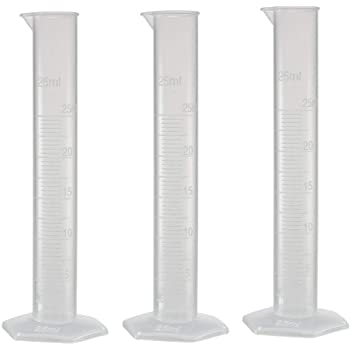
\includegraphics[width=5cm, height=5cm]{cylinders.jpg}
%%     \caption{Three graduated lab cylinders, corresponding to three
%%      eigenvectors. Prior precision eigenvalues not shown.}
%%     \label{fig:cylinder}
%% \end{figure}



\subsection{Answer to Question \ref{q:why}}\label{subsec:why}
Theorem \ref{thm:char} helps us give a compelling explanation of the
measurement clusterization we obeserved for the inverse problem of the
heat equation (Fig.~\ref{fig:}). Below, we take the following steps:
We first utilize Theorem \ref{thm:char} to understand what a D-optimal
design will look like for our relaxed model; we then argue that
although not identical, a D-optimal design for the full inverse
problem of the heat equation shares similar charachteristics to the
relaxed design; finally, we show how ...

First, recall the relevant parts of Theorem \ref{thm:char}. In our
relaxed model, for a D-optimal design $\opt$:
\begin{itemize}
  \item $\opt^*\opt$ and $\fwd\prcov \fwd^*$ are simultaneously
    diagonalizable.
  \item $\opt^*\opt$ has non-zero eigenvalues only for the $k:=\rank
    \opt^*\opt$ largest eigenvalues $\lambda_j$ of $\fwd\prcov\fwd^*$,
    i.e.~$\eta_j=0$ for $j>k$.
  \item $k$ is monotonic in $m$, the number of measurements we take.
\end{itemize}

Consider $\fwd$ and $\prcov$ from the \emph{the inverse problem of the
heat equation}. As before, we denote the eigenvalues of
$\fwd\prcov\fwd^*$ by $\lambda_j$. We input these eigenvalues into our
\emph{relaxed} model, and find a D-optimal design $\opt$ for our
relaxed model, e.g.~by using Lemma \ref{lemma:free} in the proof of
Theorem \ref{thm:char}. In our relaxed model, the measurements we take
are best utilized in reducing uncertainty for the first $k$
eigenvectors. So, a D-optimal design arising from our \emph{relaxed
model} completely avoids measuring eigenvectors $k+1$ and above.

Of course, in a real life problem --- such as the inverse problem of
the heat equation --- it is likely impossible to find measurement
locations for which all eigenvectors $k+1$ and above are
zero. Luckily, the eigenvalues of $\fwd\prcov\fwd^*$ decay very
quickly: for example, recall from Section \ref{subsec:toy} that the
eigenvalues of the forward model for the 1D heat equation are $-(2\pi
n)^{-2}$. Thus a D-optimal design is a trade-off between measuring the
small number of eigenvectors we are interested in.

We explore the abovementione trade-off for the inverse problem of the
heat equation in Fig.~\ref{fig:eigenvectors}. We allow $m=4$
measurements in $\Omega = [0,1]$ and observe that D-optimal
measurement locations are clustered at $x_1 = 0.31$ and $x_2 =
0.69$. Upon close inspection of the scaled eigenvectors of $\fwd
\prcov \fwd^*$, we first observe that eigenvectors $3$ and above have
negligible prior amplitude. Since we only have $m=4$ measurements at
our disposal, we interpret these results, following Theorem
\ref{thm:char}, as implying we should only care about measuring the
first and second eigenvectors. Then, we note the D-optimal $x_1,x_2$
present a compromise between the amplitude of the first and second
eigenvectors. For example, a measurement at $x=0.5$ would have ignored
the second eigenvector altogether, since the second eigenvector is
zero at $x=0.5$.  Now we can understand measurement clusterization:
attempting to measure what we want and ignoring the rest, along with
the spatial limitations on measurements imposed by the structure of
eigenvectors of $\fwd \prcov \fwd^*$ is the cause for measurement
clusterization in D-optimal designs: we have $m=4$ measuremnts at our
disposal but only two spatial locations that are a good compromise
between the scaled eigenvectors. Thus, clusterization arises by the
pigeonhole principle.

\begin{figure}\label{fig:eigenvectors}
    \centering
    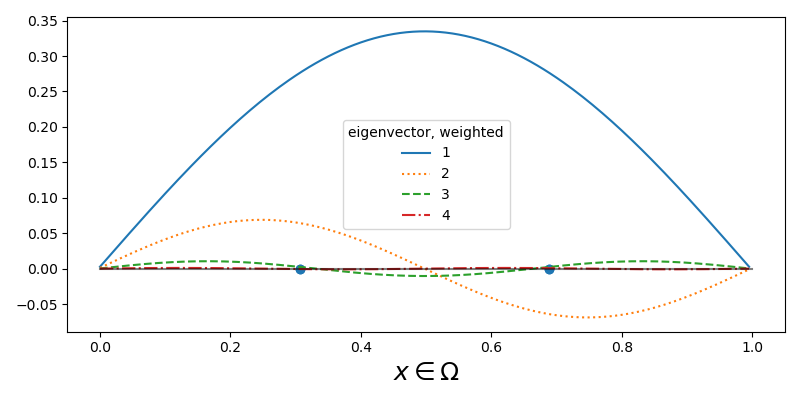
\includegraphics[width=\textwidth]{eigenvectors_dst_scaled.png}
    \caption{D-optimal measurement locations ($m=4$ measurements) and
      weighted eigenvectors for finding the initial condition of the
      1D heat equation. Measurement locations and weighted
      eigenvectors are plotted over the computational domain $\Omega =
      [0, 1]$ (x-axis). Measurement clusterization occurs
      approximately at $0.31$ and $0.69$. These two locations are a
      compromise between the magnitudes of the first and second
      eigenvectors. These are the eigenvectors a D-optimal design aims
      to measure. The rest of the eAllocating $m=4$ measurements into two locations
      results in clusterization, according to the pigeonhole
      principle.}
  \label{fig:why}
\end{figure}
\section{Numerical Experiments}
%We provide numerical evidence supporting our conclusions.


\subsection{Simulating Lemma \ref{lemma:free}}\label{subsec:lemma sims}
In the proof of Theorem \ref{thm:char} we utilize Lemma
\ref{lemma:free} to construct D-optimal designs. We implement the
construction in Lemma \ref{lemma:free} with the goal of testing
numerically how prevalent are clustered designs. We iterate over the
number of measurements $m \in \{4,\dots, 15\}$, and for every $m$ we
then iterate over $k:=\rank \obs^*\obs \in \{2,\dots, m-1\}$. For each
pair $m,k$ we run $N=5000$ simulations according to the following
steps:
\begin{enumerate}
\item Generate random diagonal $D\in \mathbb{R}^{k\times k}$ with
  entries $\log (d_i) \sim \mathcal{N}(5,1)$ and normalize it so that
  $\ttr D = m$.
\item Conjugate $D$ by a random orthogonal matrix to form a positive
  semi-definite $M := UDU^t \in \mathbb{R}^{k\times k}$.
\item Apply the construction of Lemma \ref{lemma:free} to calculate
  $A$ such that $AA^t = M$, where $A$ has unit norm columns.
\item Since columns of $A$ correspond to measurement vectors, we call
  $A$ "clustered" if $A$ has two or more identical columns (up to some
  numerical precision threshold).
\end{enumerate}
We then calculate the fraction of clustered designs of the simulations
we ran, for each pair $m,k$. Clusteriztion occured at high rates
($>95\%$) whenever $m-k > 1$; see Fig.~\ref{fig:sim AAt}. Hence, in
these simulations, clusterization is a generic property. However, when
$m-k \leq 2$, clusterization does not occur. We do not why and further
investigation into this phenomenon is out of scope for the current
study.

\begin{figure}
    \centering
    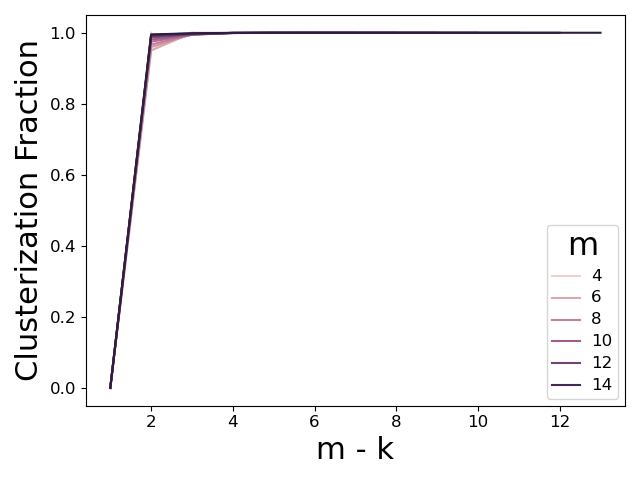
\includegraphics[height=0.5\textwidth]{simulations.png}
    \caption{Fraction of clustered $A$ for $AA^t = M$ and $M$
      generated randomly (see text and repository for details on
      generating $M$). It is evident that when $m-k >3$ clusterization
      is ubiquitous, whereas for lower $m-k$ clusterization does not
      occur.}
  \label{fig:sim AAt}
\end{figure}

Full results are located in the \texttt{simulations.csv} file within
the accompanying \href{https://github.com/yairdaon/OED}{repository},
code implementing the experiments described above is located in module
\texttt{zeros.py} of said repository.


\subsection{Correlated errors}\label{subsec:corr errors sims}
In order to verify the results of Section \ref{section:non vanishing},
we run simulations of the inverse problem of the 1D heat equation with
nonvanishing model error \(\modcov = \prcov^2 \). Indeed, including
model correlation pushes measurements apart, see Fig.~\ref{fig:corr
  errors}. Code generating Fig.~\ref{fig:corr errors} is located in
module \texttt{clusterization.py} in the accompanying
\href{https://github.com/yairdaon/OED}{repository}.

\begin{figure}
    \centering
    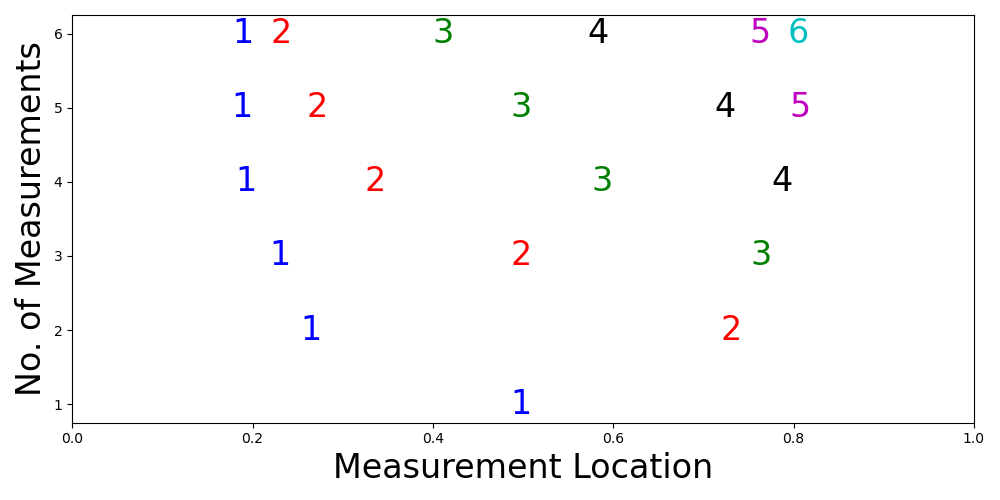
\includegraphics[height=0.5\textwidth]{dst_modelError4.png}
    \caption{Model correlation mitigates clusterization. We add a
      model correlation term to the error terms in the 1D heat
      equation inverse problem. Lo and behold, measurements are not
      close anymore and are pushed away thanks to the model error
      term.}
  \label{fig:corr errors}
\end{figure}
%\section{Answers to questions posed in the introduction}
First of all, it is important to state that we do not view measurement
clusterization as undesirable, nor do we believe it should be avoided
at all. Clusterization is a peculiar phenomenon and it is perfectly
reasonable for someone to argue against the D-optimality criterion
based on the fact that it results in clustered designs. We have seen,
however that there is perfectly reasonable explanation for
clusterization, i.e.~that clusterization arises when we seek a
designWe have shown that clusterization is an innevitable conseqeunce
of having a problem with modes of higher uncertainty than
others. Clusterization manifests the true underlying objective



\subsubsection{Answer to Question \ref{q:generic}}
We have shown through analysis and numerical experiments that



\subsubsection{Answer to Question \ref{q:mitigate}}
We have show


\subsubsection{Answer to Question \ref{q:why}}
Theorem \ref{thm:char} helps us give a compelling explanation of the
measurement clusterization we obeserved for the inverse problem of the
heat equation (Fig.~\ref{fig:}). Below, we take the following steps:
We first utilize Theorem \ref{thm:char} to understand what a D-optimal
design will look like for our relaxed model; we then argue that
although not identical, a D-optimal design for the full inverse
problem of the heat equation shares similar charachteristics to the
relaxed design; finally, we show how ...

First, recall from Theorem \ref{thm:char} that in our relaxed model,
for a D-optimal design $\opt$:
\begin{enumerate}
  \item $\opt^*\opt$ is simultaneously diagonalizable with $\fwd
    \prcov \fwd^*$.
  \item $\opt^*\opt$ has non-zero eigenvalues only for the $k:=\rank
    \opt^*\opt$ largest eigenvalues $\lambda_j$ of $\fwd\prcov\fwd^*$,
    i.e.~$\eta_j=0$ for $j>k$.
  \item $k$ is monotonic in $m$, the number of measurements we take.
\end{enumerate}

Now, consider $\fwd$ and $\prcov$ from the \emph{the inverse problem
of the heat equation}. As before, we denote the eigenvalues of
$\fwd\prcov\fwd^*$ by $\lambda_j$. We input these eigenvalues into our
\emph{relaxed} model, and find a D-optimal design $\opt$ for our
relaxed model. In our relaxed model, the measurements we take are best
utilized in reducing uncertainty for the first $k$ eigenvectors. So, a
D-optimal design arising from our \emph{relaxed model} completely
avoids measuring eigenvectors $k+1$ and above.

Of course, in a real life problem --- such as the inverse problem of
the heat equation --- it is likely impossible to find measurement
locations for which all eigenvectors $k+1$ and above are
zero. However, we can still expect a D-optimal design to give as
little weight as possible to eigenvectors $k+1$ and above. Thus a
D-optimal design is a trade-off between measuring eigenvectors we want
(eigenvectors for which $\lambda_j$ is large) and treating the rest as
noise.


We explore the abovementione trade-off for the inverse problem of the
heat equation in Fig.~\ref{fig:eigenvectors}. We allow $m=4$
measurements in $\Omega = [0,1]$ and observe that D-optimal
measurement locations are clustered at $x_1 = 0.31$ and $x_2 =
0.69$. Upon close inspection of the scaled eigenvectors of $\fwd
\prcov \fwd^*$, we first observe that eigenvectors $3$ and above have
negligible prior amplitude. Since we only have $m=4$ measurements at
our disposal, we interpret these results, following Theorem
\ref{thm:char}, as implying we should only care about measuring the
first and second eigenvectors. Then, we note the D-optimal $x_1,x_2$
present a compromise between the amplitude of the first and second
eigenvectors. For example, a measurement at $x=0.5$ would have ignored
the second eigenvector altogether, since the second eigenvector is
zero at $x=0.5$.  Now we can understand measurement clusterization:
attempting to measure what we want and ignoring the rest, along with
the spatial limitations on measurements imposed by the structure of
eigenvectors of $\fwd \prcov \fwd^*$ is the cause for measurement
clusterization in D-optimal designs: we have $m=4$ measuremnts at our
disposal but only two spatial locations that are a good compromise
between the scaled eigenvectors. Thus, clusterization arises by the
pigeonhole principle.



\begin{acks}[Acknowledgments]
This study is a result of research I started during my PhD studies
under the instruction of Prof.~Georg Stadler at the Courant Institute
of Mathematical Sciences. I would like to thank him for his great
mentorship, attention to details and kindness. I would also like to
thank Christian Remling, who helped me find a proof for Lemma
\ref{lemma:free} in
\href{https://mathoverflow.net/questions/280168/redistribute-diagonal-entries-of-a-matrix/280203#280203c}{Mathoverflow}.
Last, but certainly not least, I would like to thank the three
referees, associate editor and editor in chief for providing detailed
and insightful reviewes that have made this manuscript a whole lot
better.
%Having worked on this manuscript alone for several years, they have
%almost become my coautoh
  
This research was supported in part by an appointment with the
National Science Foundation (NSF) Mathematical Sciences Graduate
Internship (MSGI) Program sponsored by the NSF Division of
Mathematical Sciences. This program is administered by the Oak Ridge
Institute for Science and Education (ORISE) through an interagency
agreement between the U.S. Department of Energy (DOE) and NSF. ORISE
is managed for DOE by ORAU. All opinions expressed in this paper are
the author's and do not necessarily reflect the policies and views of
NSF, ORAU/ORISE, or DOE.
% This work was also supported by The Raymond and Beverly Sackler
% Post-Doctoral Scholarship.
\end{acks}

\bibliographystyle{ba}
\bibliography{../../lib.bib}


\end{document}

